\\for con
\#TODO
I have introduced a new architecture called Var-Casper, which is one of the constructive cascade neural networks with variational encoding inputs [1]. In this article I have a quick review on the topology of Casper and VAE, and also try to apply Var-Casper on SARS dataset in order to exceed the patient classification algorithm by CasCor in my previous work. It seems that the result of Var-Casper has an edge over my previous work CasCor model by around 25\% test accuracy increase in SARS dataset. Therefore, this model can be more efficient for people to check the self-risk of SARS or other diseases since it only requires body temperature data. Also, it is a light neuron network that does not require much space and computational power [11] (like GPT-3) to boost the prediction performance. The main point of Var-Casper is it can automatically match the network complexity to the problem true complexity by adding highly correlated feature extractors, or frozen hidden neurons. Because the hidden neurons can quickly learn from data by a large learning rate while they are firstly added, the Var-Casper can easily extract features via optimizing the hidden to output weights. Var-Casper can also save training time since the network architecture is simple at the beginning and will grow depending on the problem complexity. The Var-Casper algorithm also faces problems such as accuracy drops due to bad feature extractors, and unlike CasCor, Var-Casper can improve these bad neurons in the following epochs by a small learning rate. 
   In the future I am going to explore more difficult classification problem to explore the limit of Var-Casper. The classification problem I analyse here is quite simple for Var-Casper and can not reveal many drawbacks of the model. One of the possible improvements to solve the accuracy drop problem is to use early-stopping and evaluation of the latest hidden neuron. Also, a good initialisation algorithm may be introduced to prevent performance drops due to the bad initialised hidden neurons. Additionally, the dimension of the data can be further pruned, masked to challenge the model. Since there are 4000 datapoints in SARS-CoV-1 dataset, it’s possible to explore the few-shot learning [12]and transfer learning [13]. And it’s another improvement to be made that we can try different optimizing strategy like Adam [14]
In conclusion, Var-Casper is a dynamic generative neuron network strategy which is timesaving, robust to sparse data and highly matches the complexity of the real-world problems. It’s also shown that Var-Casper can ultimately solve SARS classification problem in current dataset with 100% accuracy.

\\for res
\# TODO change chart img to chart latex
\begin{align*}
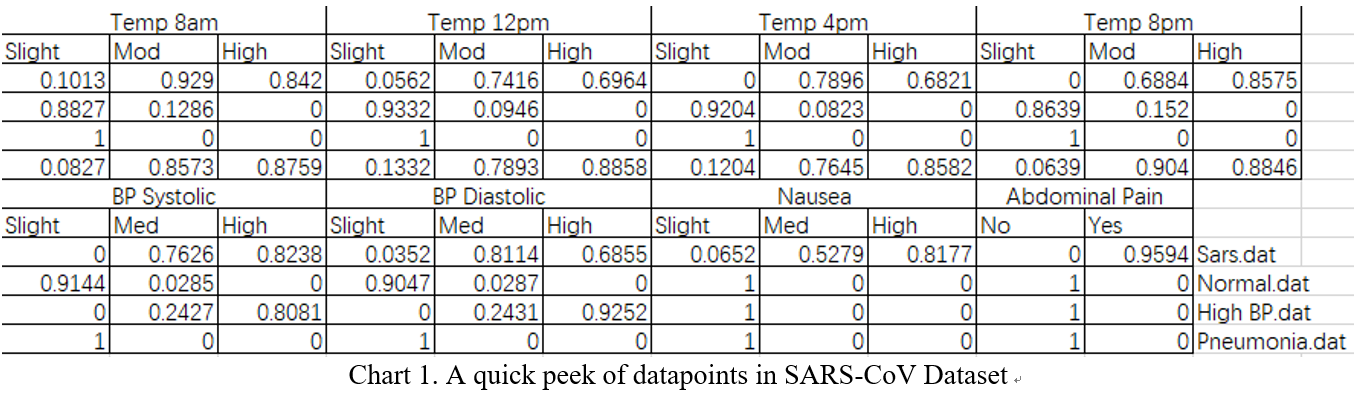
\includegraphics[width=\textwidth]{images/img6.png}    
\end{align*}
